\usepackage{figures/tikzit}
\usepackage{graphicx}
\usepackage{amssymb}
\usepackage{xparse}

\input{macros/sets}
\input{macros/category}
\input{macros/circuits}
\input{macros/streams}

\graphicspath{{./imgs/}}

\usetheme[
  background=light,
  numbering=counter,
  block=fill,
  %sectionpage=simple
]{metropolis}

\input{figures/circuits.tikzstyles}
\input{figures/circuits.tikzdefs}

% FiraFonts
\usepackage[sfdefault]{FiraSans}
\usepackage{FiraMono}
% Use thinner fonts
\makeatletter
\def\bfseries@sf{medium}
\def\mdseries@sf{l}
\makeatother

\definecolor{backg}{RGB}{9,72,61}
\definecolor{accent}{RGB}{0,150,136}

\definecolor{dracback}{RGB}{40, 42, 54}
\definecolor{dracfore}{RGB}{248, 248, 242}
\definecolor{dractitle}{RGB}{56, 58, 89}
\definecolor{dracblock}{RGB}{98, 114, 164}
\definecolor{draccent}{RGB}{255, 121, 198}

\setbeamercolor{normal text}{bg=dracfore}
\setbeamercolor{frametitle}{bg=dractitle, fg=dracfore}
\setbeamercolor{title separator}{fg=draccent}
\setbeamercolor{progress bar}{fg=draccent, bg=draccent}
\setbeamercolor{block title}{fg=dracfore, bg=dracblock}
\setbeamercolor{alerted text}{fg=draccent}

\newtheorem{axiom}{Axiom(s)}

\title{Rewriting modulo traced comonoid structure}
\author{
    \texorpdfstring{
        \large \textbf{George Kaye}
    }{
        George Kaye
    }
    \and
    \texorpdfstring{
        \large Dan Ghica
    }{
        Dan Ghica
    }
}
\date{
    \texorpdfstring{
        University of Birmingham
    }{
        04 July 2023
    }
}
\institute{
    \texorpdfstring{
        \normalsize 04 July 2023 -- FSCD 2023, Rome
    }{
        University of Birmingham
    }
}

\begin{document}
    \maketitle

    \begin{frame}
    \frametitle{Why are we here?}

    \centering
    \LARGE

    We want to reason \alert{equationally} with \alert{processes} with notions of
    \alert{feedback}, \alert{copying} and \alert{discarding}

    \normalsize
    (e.g.\ \alert{digital circuits})

    \large
    \pause

    \vspace{1em}

    What should the \alert{syntax} for these processes be?

    \pause

    How do we \alert{reason} with this syntax?

    \pause

    What is the best way to \alert{rewrite} with this syntax?

    \pause

    Is this syntax suitable for \alert{automating} rewrites?

\end{frame}
\begin{frame}
    \frametitle{The building blocks}

    \centering

    \pause
    \LARGE
    The graphical syntax of \alert{string diagrams}

    \pause
    \normalsize
    \vspace{2em}

    \dsptikzfig{strings/category/f}[f][white][m][n]
    \dsptikzfig{strings/category/f}[g][white][n][p]

    \pause
    \vspace{2em}

    \dsptikzfig{strings/category/composition}[f][g][white][m][n][p]
    \dsptikzfig{strings/monoidal/tensor}[f][g][white][m][n][n][p]
    \pause
    \dsptikzfig{strings/category/identity}[white][m]
    \dsptikzfig{strings/symmetric/symmetry}[white][m][n]

    \normalsize
    \vspace{1em}

    (\alert{symmetric monoidal category})

\end{frame}

\begin{frame}
    \frametitle{Why are we here?}

    \centering
    \LARGE
    We want to have \alert{feedback}.

    \pause
    \normalsize
    \vspace{2em}

    \dsptikzfig{strings/category/f-2-2}[f][white][x][m][x][n]
    \quad
    \pause
    \scalebox{2}{\(\Rightarrow\)}
    \quad
    \dsptikzfig{strings/traced/trace-rhs}[f][white][m][n][x]

    \pause
    \vspace{1em}
    (traced structure)

\end{frame}

\begin{frame}
    \frametitle{Why are we here?}

    \centering

    \LARGE
    We want to \alert{fork} and \alert{stub}.

    \pause

    \normalsize
    \vspace{1em}

    \dsptikzfig{strings/structure/comonoid/copy}[white]
    \dsptikzfig{strings/structure/comonoid/discard}[white]

    \newcommand{\comonscale}{0.75}
    \begin{gather*}
        \scalebox{\comonscale}{\dsptikzfig{strings/structure/comonoid/unitality-l-lhs}}
        =
        \scalebox{\comonscale}{\dsptikzfig{strings/structure/comonoid/unitality-l-rhs}}
        \qquad
        \scalebox{\comonscale}{\dsptikzfig{strings/structure/comonoid/unitality-r-lhs}}
        =
        \scalebox{\comonscale}{\dsptikzfig{strings/structure/comonoid/unitality-r-rhs}}
        \qquad
        \scalebox{\comonscale}{\dsptikzfig{strings/structure/comonoid/associativity-lhs}}
        =
        \scalebox{\comonscale}{\dsptikzfig{strings/structure/comonoid/associativity-rhs}}
        \qquad
        \scalebox{\comonscale}{\dsptikzfig{strings/structure/comonoid/commutativity-lhs}}
        =
        \scalebox{\comonscale}{\dsptikzfig{strings/structure/comonoid/commutativity-rhs}}
    \end{gather*}

    \pause
    \vspace{1em}
    (commutative comonoid structure)

\end{frame}

\begin{frame}
    \frametitle{Why are we here?}

    \centering

    \LARGE
    We want to \alert{copy} and \alert{discard}.

    \normalsize
    \pause
    \begin{gather*}
        \dsptikzfig{strings/structure/cartesian/naturality-copy-lhs}[f][white]
        =
        \dsptikzfig{strings/structure/cartesian/naturality-copy-rhs}[f][white]
        \qquad
        \dsptikzfig{strings/structure/cartesian/naturality-discard-lhs}[f][white]
        =
        \dsptikzfig{strings/structure/cartesian/naturality-discard-rhs}
    \end{gather*}

    \pause
    \vspace{1em}
    (Cartesian structure)

\end{frame}

\begin{frame}
    \frametitle{Why are we here?}

    \centering

    \LARGE
    We want to reason \alert{graphically}.
    \normalsize

    \pause
    \visible<2->{\dsptikzfig{strings/dataflow/unfolding-animation/step-0-nobox}[F][white]}
    \visible<3->{\(=\)}
    \visible<3>{\only<1-3>{\dsptikzfig{strings/dataflow/unfolding-animation/step-1}[F][white]}}%
    \only<4>{\dsptikzfig{strings/dataflow/unfolding-animation/step-2}[F][white]}%
    \only<5>{\dsptikzfig{strings/dataflow/unfolding-animation/step-3}[F][white]}%
    \only<6>{\dsptikzfig{strings/dataflow/unfolding-animation/step-4}[F][white]}%
    \only<7>{\dsptikzfig{strings/dataflow/unfolding-animation/step-5}[F][white]}%
    \only<8->{\dsptikzfig{strings/dataflow/unfolding-animation/step-6}[F][white]}%

    \visible<9>{(unfolding, fixpoint equation)}

\end{frame}

\begin{frame}
    \frametitle{Why are we here?}

    \center

    \LARGE
    We want to do this reasoning \alert{computationally}.

    \pause
    \vspace{0.5em}

    This is \alert{hard} for terms, even with string diagrams.

    \normalsize
    (lots of shuffling around and bookkeeping required)
    \LARGE

    \pause
    \vspace{0.5em}
    But computers like \alert{graphs}...

\end{frame}
    % !TeX root = ../main-presentation.tex
\begin{frame}
    \frametitle{What came before}

    \pause
    \centering
    \LARGE
    String graphs
    \raisebox{-2em}{
        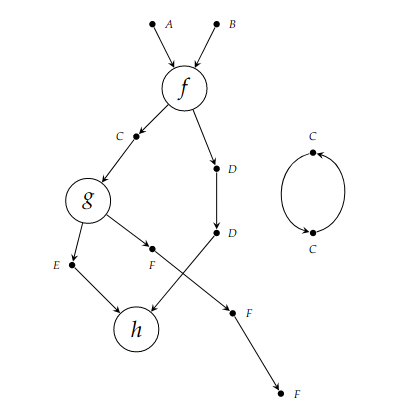
\includegraphics[width=0.2\textwidth]{string-graphs}
    }

    \pause
    \normalsize
    \vspace{1em}
    Dixon, Kissinger

    
\includegraphics[width=0.15\textwidth]{dixon}
    
\includegraphics[width=0.15\textwidth]{kissinger}

\end{frame}

\begin{frame}
    \frametitle{What came before}

    \pause
    \centering
    \LARGE
    Hypergraphs
    \quad
    \raisebox{-1.5em}{
        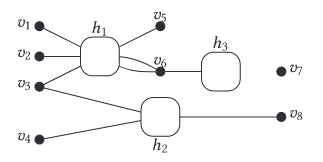
\includegraphics[width=0.3\textwidth]{hypergraphs}
    }

    \pause
    \normalsize
    \vspace{1em}
    Bonchi, Gadduchi, Kissinger, Sobocinski, Zanasi

    \hypergraphpeople

\end{frame}

\begin{frame}
    \frametitle{The hyper kind of graph}

    \centering
    \dsptikzfig{graphs/example}

\end{frame}

\begin{frame}
    \frametitle{The hyper kind of (interfaced) graph}

    \centering
    \dsptikzfig{graphs/example-cospan}

\end{frame}

\begin{frame}
    \frametitle{Terms to graphs}

    \centering
    \LARGE

    \textbf{Goal}

    Interpret \alert{string diagrams} as \alert{cospans of hypergraphs}

    \vspace{1em}
    \pause

    But which hypergraphs?

\end{frame}

\begin{frame}
    \frametitle{Feeling special}

    \centering

    \Large
    Which terms correspond to cospans of hypergraphs?

    \pause

    \normalsize
    Special commutative Frobenius structure

    \pause
    \normalsize
    \vspace{1em}
    \dsptikzfig{strings/structure/monoid/init}[white]
    \dsptikzfig{strings/structure/comonoid/copy}[white]
    \dsptikzfig{strings/structure/monoid/merge}[white]
    \dsptikzfig{strings/structure/comonoid/discard}[white]
    \pause
    \vspace{1em}

    Any category with this structure is \alert{self-dual compact closed}
    \pause
    \[
        \dsptikzfig{strings/compact-closed/cup}
        :=
        \dsptikzfig{strings/structure/monoid/init}[white]
        \scalebox{1.5}{\(\seq\)}
        \dsptikzfig{strings/structure/comonoid/copy}[white]
        \qquad
        \dsptikzfig{strings/compact-closed/cap}
        :=
        \dsptikzfig{strings/structure/monoid/merge}[white]
        \scalebox{1.5}{\(\seq\)}
        \dsptikzfig{strings/structure/comonoid/discard}[white]
    \]

\end{frame}

\begin{frame}
    \frametitle{Feeling special}

    \centering

    Modulo some equations...
    \newcommand{\frobscale}{0.75}
    \begin{gather*}
        \scalebox{\frobscale}{\dsptikzfig{strings/structure/monoid/unitality-l-lhs}}
        =
        \scalebox{\frobscale}{\dsptikzfig{strings/structure/monoid/unitality-l-rhs}}
        \qquad
        \scalebox{\frobscale}{\dsptikzfig{strings/structure/monoid/unitality-r-lhs}}
        =
        \scalebox{\frobscale}{\dsptikzfig{strings/structure/monoid/unitality-r-rhs}}
        \qquad
        \scalebox{\frobscale}{\dsptikzfig{strings/structure/monoid/associativity-lhs}}
        =
        \scalebox{\frobscale}{\dsptikzfig{strings/structure/monoid/associativity-rhs}}
        \qquad
        \scalebox{\frobscale}{\dsptikzfig{strings/structure/monoid/commutativity-lhs}}
        =
        \scalebox{\frobscale}{\dsptikzfig{strings/structure/monoid/commutativity-rhs}}
        \\[1em]
        \scalebox{\frobscale}{\dsptikzfig{strings/structure/comonoid/unitality-l-lhs}}
        =
        \scalebox{\frobscale}{\dsptikzfig{strings/structure/comonoid/unitality-l-rhs}}
        \qquad
        \scalebox{\frobscale}{\dsptikzfig{strings/structure/comonoid/unitality-r-lhs}}
        =
        \scalebox{\frobscale}{\dsptikzfig{strings/structure/comonoid/unitality-r-rhs}}
        \qquad
        \scalebox{\frobscale}{\dsptikzfig{strings/structure/comonoid/associativity-lhs}}
        =
        \scalebox{\frobscale}{\dsptikzfig{strings/structure/comonoid/associativity-rhs}}
        \qquad
        \scalebox{\frobscale}{\dsptikzfig{strings/structure/comonoid/commutativity-lhs}}
        =
        \scalebox{\frobscale}{\dsptikzfig{strings/structure/comonoid/commutativity-rhs}}
        \\[1em]
        \scalebox{\frobscale}{\dsptikzfig{strings/structure/frobenius/frobenius-l}}
        =
        \scalebox{\frobscale}{\dsptikzfig{strings/structure/bialgebra/merge-copy-lhs}}
        \qquad
        \scalebox{\frobscale}{\dsptikzfig{strings/structure/frobenius/frobenius-r}}
        =
        \scalebox{\frobscale}{\dsptikzfig{strings/structure/bialgebra/merge-copy-lhs}}
        \qquad
        \scalebox{\frobscale}{\dsptikzfig{strings/structure/frobenius/copy-merge-lhs}}
        =
        \scalebox{\frobscale}{\dsptikzfig{strings/structure/frobenius/copy-merge-rhs}}
    \end{gather*}
\end{frame}

\begin{frame}
    \frametitle{Feeling special graphs}

    \centering

    \begin{minipage}{0.45\textwidth}
        \begin{center}
            isomorphism class of hypergraphs

            \vspace{1em}

            \scalebox{0.625}{\dsptikzfig{graphs/example-frobenius-cospan}}
        \end{center}
    \end{minipage}
    \quad
    \raisebox{-1em}{\(\leftrightarrow\)}
    \pause
    \begin{minipage}{0.45\textwidth}
        \begin{center}
            Frobenius term modulo equations

            \vspace{1em}

            \dsptikzfig{graphs/example-frobenius-term}
        \end{center}
    \end{minipage}

    \vspace{1em}
    \normalsize
    \scalebox{0.75}{\hypergraphpeople}

    \Large
    \pause
    So vanilla hypergraphs are \alert{not restrictive enough}.

\end{frame}

\begin{frame}
    \frametitle{Take a step back}

    \pause

    \centering
    \LARGE
    \alert{Monogamy}

    \scalebox{0.5}{\hypergraphpeople}

    \pause
    \normalsize

    One connection on the \alert{left}, one on the \alert{right}

    \pause
    \vspace{1em}

    \scalebox{0.9}{
        \dsptikzfig{graphs/identity}
        \qquad
        \dsptikzfig{graphs/composition}
    }

\end{frame}
\begin{frame}
    \frametitle{A bit too special}

    \centering

    \begin{minipage}{0.45\textwidth}
        \begin{center}
            \alert{monogamous acyclic} hypergraphs

            \vspace{1em}

            \scalebox{0.625}{\dsptikzfig{graphs/example-monogamous-acyclic}}
        \end{center}
    \end{minipage}
    \quad
    \raisebox{-1em}{\(\leftrightarrow\)}
    \pause
    \begin{minipage}{0.45\textwidth}
        \begin{center}
            symmetric monoidal term

            \vspace{1em}

            \dsptikzfig{graphs/example-smc-term}
        \end{center}
    \end{minipage}

    \vspace{1em}
    \normalsize
    \scalebox{0.75}{\hypergraphpeople}

    \Large
    \pause
    Monogamous acyclic hypergraphs are \alert{too restrictive}.

\end{frame}

\begin{frame}
    \frametitle{Frobenius to traced comonoid}

    \centering
    \vspace{0.5em}
    \Large
    Traced comonoid is `half' Frobenius...

    \normalsize

    \dsptikzfig{strings/structure/comonoid/copy}[white]
    \dsptikzfig{strings/structure/comonoid/discard}[white]

    \pause

    \vspace{1em}

    \Large
    Trace built from compact closed structure...
    \[
        \begin{array}{c}
            \dsptikzfig{strings/compact-closed/cup}[white]
            \\
            \tensor
            \\
            \dsptikzfig{strings/category/identity}[white]
        \end{array}
        \seq
        \begin{array}{c}
            \dsptikzfig{strings/category/identity}[white]
            \\
            \tensor
            \\
            \dsptikzfig{strings/category/f-2-2}[f][white]
        \end{array}
        \seq
        \begin{array}{c}
            \dsptikzfig{strings/compact-closed/cap}[white]
            \\
            \tensor
            \\
            \dsptikzfig{strings/category/identity}[white]
        \end{array}
    \]
\end{frame}

\begin{frame}
    \frametitle{Monogamous on one side}

    \centering

    \LARGE
    \alert{Partial left}-monogamy

    \scalebox{0.5}{\meanddan}

    \pause
    \normalsize

    One connection on the \alert{left}, many on the \alert{right}

    \pause
    \scalebox{0.9}{
        \dsptikzfig{graphs/fork-cospan}
        \qquad
        \dsptikzfig{graphs/stub-cospan}
    }

    \scalebox{0.9}{
        \dsptikzfig{graphs/fork-edge-cospan}
        \qquad
        \dsptikzfig{graphs/fork-interface-edge-cospan}
    }
\end{frame}

\begin{frame}
    \frametitle{Hold on a moment}

    \centering
    \pause
    \LARGE
    \alert{Special cases...}

    \Large
    \pause
    \vspace{0.5em}

    Trace of the identity

    \vspace{0.5em}

    \scalebox{0.8}{
        \dsptikzfig{graphs/trace-identity}
        \dsptikzfig{graphs/trace-identity-cospan}
    }

    \vspace{0.5em}

    Trace of the fork

    \vspace{0.5em}

    \scalebox{0.8}{
        \dsptikzfig{graphs/trace-fork}
        \dsptikzfig{graphs/trace-fork-cospan}
    }
\end{frame}

\begin{frame}
    \frametitle{The correspondence}

    \centering

    \begin{minipage}{0.45\textwidth}
        \begin{center}
            partial left-monogamous hypergraphs
            \vspace{1em}

            \scalebox{0.625}{\dsptikzfig{graphs/example-trace-cospan}}
        \end{center}
    \end{minipage}
    \pause
    \quad
    \raisebox{-1em}{\(\leftrightarrow\)}
    \begin{minipage}{0.45\textwidth}
        \begin{center}
            traced comonoid term

            \vspace{1em}

            \dsptikzfig{graphs/example-trace-term}
        \end{center}
    \end{minipage}

    \pause
    \vspace{1.5em}

    \meanddan

\end{frame}
\end{document}